\startchapter{Channel Modeling}
\label{chapter:Mod}
In this section, I modeled communication channels in the traces. There are two model, guaranteed communication model and in-guaranteed communication model. For both of these two model the communication consist of three stages: 1. channel opening, 2. data exchanging and 3. channel closing.

\section{Communications Stages}   
A communication in this work is happen in a channel. There are 3 main stages of a communication in this model: 1. open the channel, 2. message send/receive, 3. close the channel. Figure \ref{communicationhappen} indicate how communications happen between two ends of both sides of a channel. In the open channel stage, each end need to call its own channel open functions. This open function might be one or more functions which can be channel create function, open function, connect function etc.  In the message send/receive stage, messages are being sent into the channel in one side and received in the other side. In the final channel close stage, the channel delete function, disconnect function, close function etc. will be called. The channel can be reopen again to start new communications after the close stage. However the reopen channel will be treated as a communication cycle.

The operations being concerned in this model are: channel open in sender side, channel open in the receiver side, message send, message receive, channel close in sender side, channel close in receiver side. The number of send and receive function calls for one message do not necessary to be the same. It can be one to one, one to multiple, multiple to one, or multiple to multiple. Both sides of the channel shared the same channel name but different channel handle for its own operations.

\begin{figure}[h]
\centerline{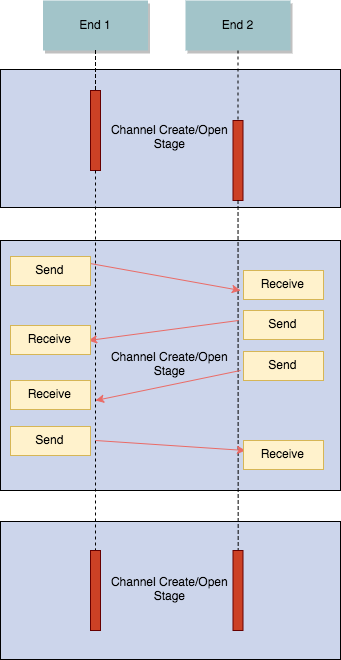
\includegraphics[scale=0.6]{Figures/communicationhappen}}
 \caption{Communication Model}
\label{communicationhappen}
\end{figure}


\section{Communication Scenarios}
Both the order guaranteed communication model and the order in-guaranteed communication model contains several send/receive scenarios. Table \ref{scenarios_g} shows all of send/receive scenarios for guaranteed communication model while Table \ref{scenarios_ig} shows all of send/receive scenarios for in-guaranteed communication model.


\begin{longtable}{|c|c|p{6.5cm}|}
\caption{Send/Receive Scenarios of Order Guaranteed Communication Model}\label{scenarios_g}\\
\hline
\textbf{Scenario} & \textbf{Diagram} & \textbf{Comment}\\ \hline
 1 &\raisebox{-\totalheight}{ 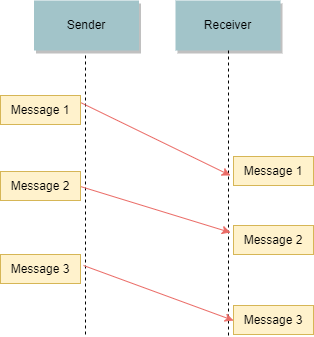
\includegraphics[scale=0.3]{Figures/scenario1}} & Message send/receive successfully in order                       \\ \hline
 3 &\raisebox{-\totalheight}{  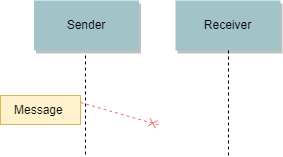
\includegraphics[scale=0.3]{Figures/scenario3}} &  Message send/receive fail \\ \hline
 4 & \raisebox{-\totalheight}{ 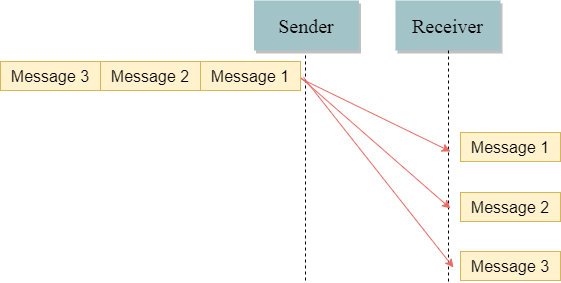
\includegraphics[scale=0.3]{Figures/scenario4}} & One sent message received segmented \\ \hline
 6 & \raisebox{-\totalheight}{ 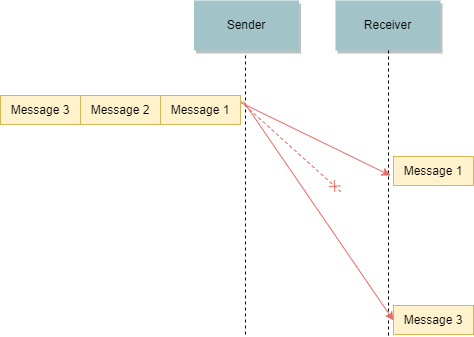
\includegraphics[scale=0.3]{Figures/scenario6}}  &  One sent message received segmented in order, but partially lost \\ \hline
 8 & \raisebox{-\totalheight}{ 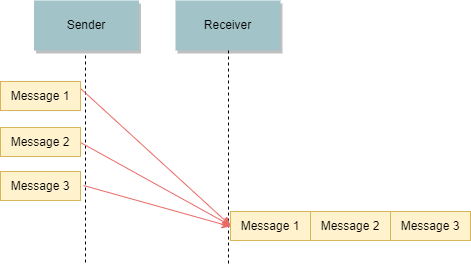
\includegraphics[scale=0.3]{Figures/scenario8}}  & Multiple messages received at a time \\ \hline
 9 & \raisebox{-\totalheight}{ 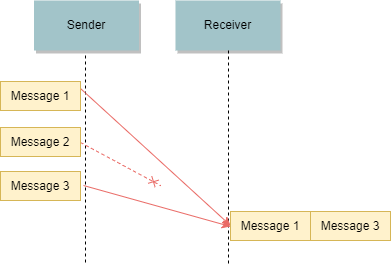
\includegraphics[scale=0.3]{Figures/scenario9}}  & Multiple messages received at a time, but partially lost \\\hline
 10 & \raisebox{-\totalheight}{ 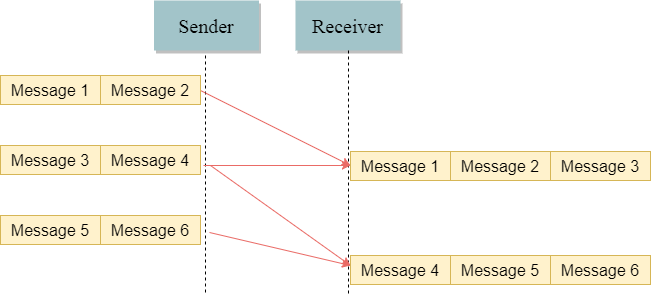
\includegraphics[scale=0.3]{Figures/scenario10}} &  Messages segmented and reconstructed in order \\ \hline
 12 & \raisebox{-\totalheight}{ 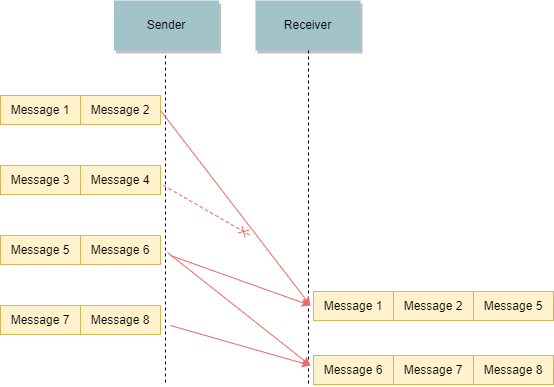
\includegraphics[scale=0.3]{Figures/scenario12}} & Messages segmented and reconstructed partially lost \\ \hline
\end{longtable}

\begin{longtable}{|c|c|p{6.5cm}|}
\caption{SSend/Receive Scenarios of Order In-Guaranteed Communication Model}\label{scenarios_ig}\\
\hline
\textbf{Scenario} & \textbf{Diagram} & \textbf{Comment}\\ \hline
 1 &\raisebox{-\totalheight}{ 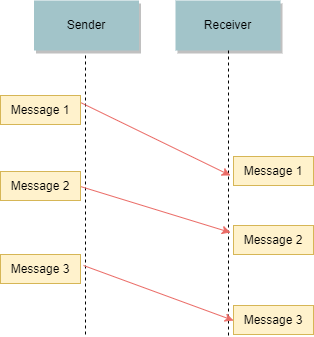
\includegraphics[scale=0.3]{Figures/scenario1}} & Message send/receive successfully in order                       \\ \hline
 2 & \raisebox{-\totalheight}{ 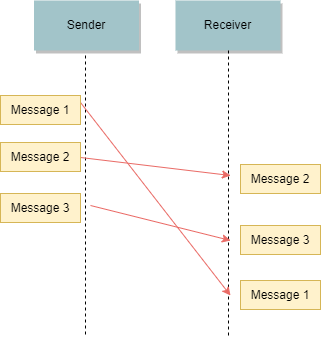
\includegraphics[scale=0.3]{Figures/scenario2}}  & Message send/receive successfully but out of order \\ \hline
 3 &\raisebox{-\totalheight}{  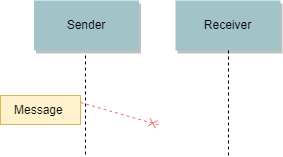
\includegraphics[scale=0.3]{Figures/scenario3}} &  Message send/receive fail \\ \hline
 4 & \raisebox{-\totalheight}{ 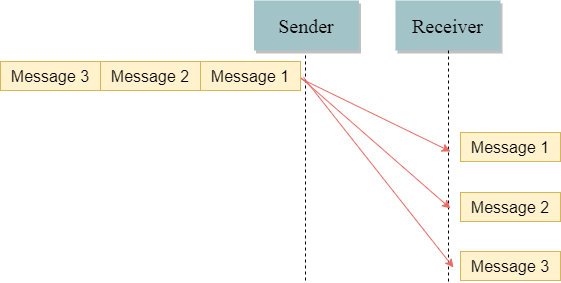
\includegraphics[scale=0.3]{Figures/scenario4}} & One sent message received segmented \\ \hline
 5 & \raisebox{-\totalheight}{ 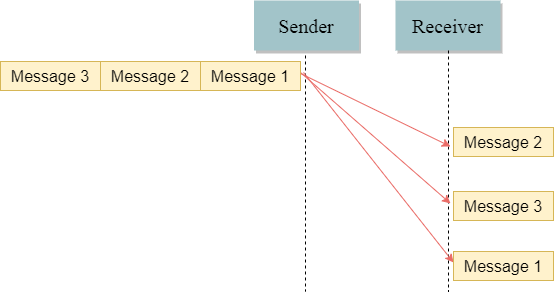
\includegraphics[scale=0.3]{Figures/scenario5}}  & One sent message received segmented and out of order \\ \hline
 6 & \raisebox{-\totalheight}{ 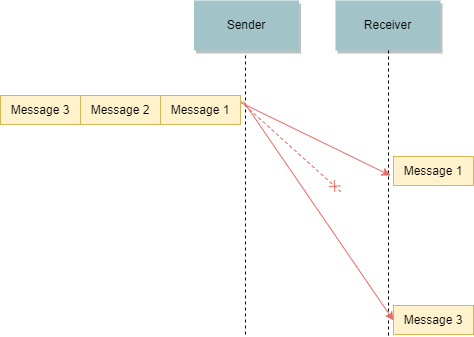
\includegraphics[scale=0.3]{Figures/scenario6}}  &  One sent message received segmented in order, but partially lost \\ \hline
 7 & \raisebox{-\totalheight}{ 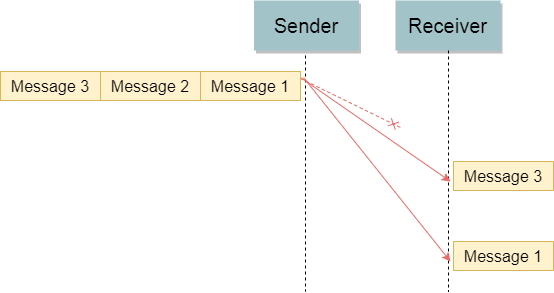
\includegraphics[scale=0.3]{Figures/scenario7}}  & One sent message received segmented out of order and partially lost \\ \hline
 8 & \raisebox{-\totalheight}{ 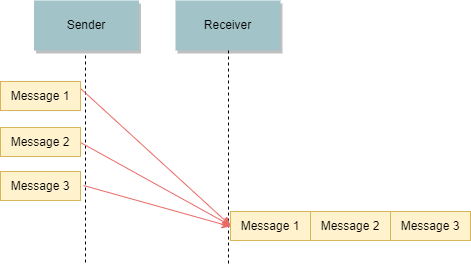
\includegraphics[scale=0.3]{Figures/scenario8}}  & Multiple messages received at a time \\ \hline
 9 & \raisebox{-\totalheight}{ 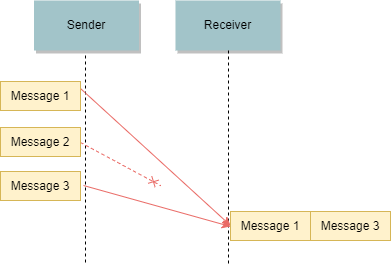
\includegraphics[scale=0.3]{Figures/scenario9}}  & Multiple messages received at a time, but partially lost \\\hline
 10 & \raisebox{-\totalheight}{ 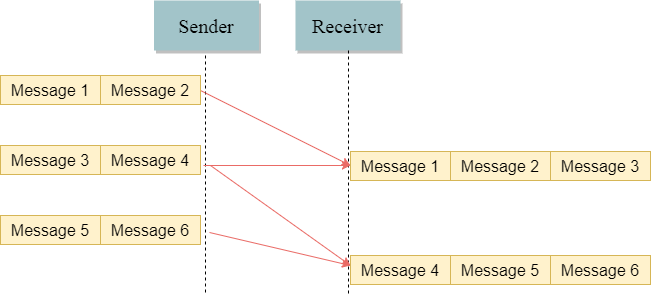
\includegraphics[scale=0.3]{Figures/scenario10}} &  Messages segmented and reconstructed in order \\ \hline
 11 & \raisebox{-\totalheight}{ 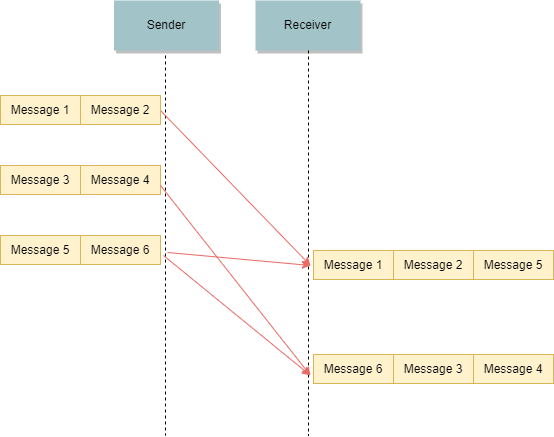
\includegraphics[scale=0.3]{Figures/scenario11}} &  Messages segmented and reconstructed out of order \\ \hline
 12 & \raisebox{-\totalheight}{ 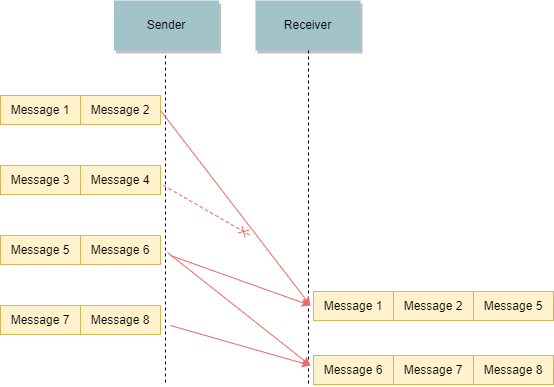
\includegraphics[scale=0.3]{Figures/scenario12}} & Messages segmented and reconstructed partially lost \\ \hline
 13 & \raisebox{-\totalheight}{ 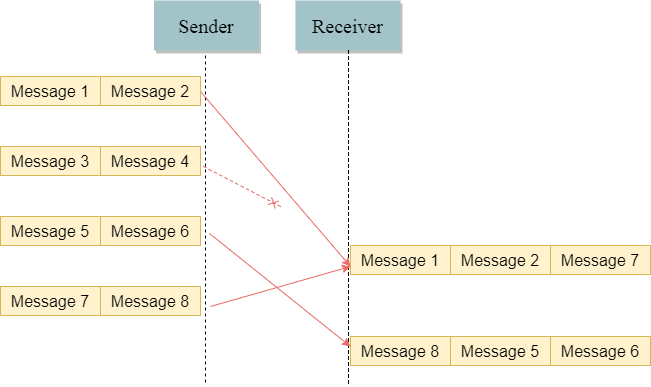
\includegraphics[scale=0.3]{Figures/scenario13}} & Messages segmented and reconstructed out of order and partially lost \\ \hline
\end{longtable}




